\chapter{Commands}

Commands can be used to do all sorts of things in phrases and tables. It is a good idea to skim through this chapter at least once, to get an idea of what they can do.


\includegraphics[width=0.84cm]{tip}TIP!
\begin{itemize}
        \item \textit{Tapping \textsc{a,a} on a command shows a scrolling help text in the top of the screen. \textsc{A+l/r} can then be used to browse through the commands. Pause the scrolling text by holding \textsc{select}.}
\end{itemize}

\section{A: Table Start/Stop}

Starts or stops tables in the current channel. Use the table number you want to start, or 20 for stopping.

\begin{description}
\item[A03] start table 3
\item[A20] stop table
\end{description}

\section{B: MayBe}

\subsection{In Phrases (MayBe Play Note)}

Controls how likely it is that the note
or sample(s) to the left will be played.
First digit sets probability for left kit,
second digit sets probability for notes
and right kit.

\begin{description}
    \item[B00] Never play note
    \item[B0F] Always play note/right kit sample
    \item[BF0] Always play note/left kit sample
    \item[B08] Play note/right kit sample about 50\% of the time
\end{description}

\subsection{In Tables (MayBe Hop)}

A hop that only happens sometimes.
First digit sets probability, second digit
sets destination row.

\begin{description}
    \item[BF5] Hop to row 5, 15 times out of 16
    \item[B84] Hop to row 4, about 50\% of the time
    \item[B03] Never hop to row 3
\end{description}

\section{C: Chord}

\subsection{For Pulse and Wave Instruments:}

\label{command-chord}
Runs an arpeggio that extends the base note with the given semitones. The speed may be slowed down using \textsc{cmd/rate} in instrument screen.

\begin{description}
\item[C37] plays a minor chord: 0, 3, 7, 0, 3, 7, 0, 3, 7, \ldots
\item[C47] plays a major chord: 0, 4, 7, 0, 4, 7, 0, 4, 7, \ldots
\item[C0C] plays 0, 0, C, 0, 0, C, 0, 0, C, \ldots
\item[CC0] plays 0, C, 0, C, 0, C, \ldots
\item[CCC] plays 0, C, C, 0, C, C, 0, C, C, \ldots
\item[C00] resets chord
\end{description}

\subsection{For Noise Instruments:}

Applies S command with the given value every second tick.

\section{D: Delay}

Delay the triggering of a note with the given number of ticks.

\section{E: Amplitude Envelope}

\subsection{For Pulse and Noise Instruments}
The first value digit sets the initial amplitude (0=min, \$F=max); the second digit sets the release (0,8: no change, 1-7: decrease, 9-\$F: increase).

\subsection{For Wave Instruments}
\begin{description}
\item[E00] volume 0\%
\item[E01] volume 25\%
\item[E02] volume 50\%
\item[E03] volume 100\%
\end{description}

\section{F: Wave Frame/Finetune}

\subsection{For Pulse Instruments:}
The first digit sets \textsc{pu2 tsp.}, the second \textsc{finetune}.
See section~\ref{detune}.

\subsection{For Kit Instruments:}
Modifies the sample position. \$00-\$7F steps forward, \$80-\$FF steps back.

\subsection{For Wave Instruments:}
Change the wave frame being played on the wave channel. This command is relative, meaning that the value is added to the current frame number. It can be used for playing through synth sounds manually.


\includegraphics[width=0.84cm]{tip}TIP!
\begin{itemize}
        \item \textit{Since a synth sound contains 16 (\$10) waves, issuing the command \textsc{F10} jumps to the next synth sound.}
	%\marginpar{
\includegraphics[width=0.84cm]{tip}TIP!}
	\end{itemize}

\begin{description}
\item Example:
\item[F01] If wave frame 3 is being played, advance 1 frame and start playing frame number 4.
\end{description}

\section{G: Groove Select}

Select the groove to use when playing phrases or tables.

\begin{description}
\item Example:
\item[G04] select groove 4
\end{description}

\section{H: Hop}

H hops to a new play position. It can also be used to stop playing.

\subsection{H in Phrases}

\begin{description}
    \item[H00-H0F] Hop to next phrase. The digit sets destination phrase step.
    \item[H10-HFE] Hop back within the phrase. The first digit sets number of times to hop back, the second digit sets destination step.
    \item[HFF] Stop playing song (or channel, if in live mode).
\end{description}


\includegraphics[width=0.84cm]{tip}TIP!
\nolinebreak
\begin{itemize}
        \item \textit{To compose in waltz time (3/4), put \textsc{H00} commands on step \textsc{C} in every phrase.}
\end{itemize}

\subsection{H in Tables}

In the table screen, H is used for creating table loops. The first digit sets how many times the hop should be done before moving on; 0 means ``forever.'' The second digit sets the table step to jump to. Loops can be nested; that is, you can have smaller loops inside bigger ones.

\begin{description}
\item Example:
\item[H21] hop twice to table position 1.
\item[H04] hop to table position 4 forever.
\end{description}

\section{K: Kill Note}

K instantly stops the sound, causing an audible click. If the click is not desired, better options might be E00 for wave channel and E11 for pulse and noise channels.

\begin{description}
\item Example:
\item[K00] kill note instantly
\item[K03] kill note after 3 ticks
\end{description}

\section{L: Slide}

Slides to the target note in the given duration. If the instrument's \textsc{pitch} setting is \textsc{tick}, the duration is given in ticks, otherwise in n/360 seconds.

Example:

\begin{verbatim}
  C-4 ---
  F-4 L40
  --- ---
  C-4 L10
\end{verbatim}

This will result in a slide that starts with C-4, bends to F-4, and then quickly bends back to C-4.

\subsection{L in Tables}

The L command may be used in the left table command column. The transpose column will then set target note relative to the base note.

\begin{figure}[htbp]
	\begin{center}
		\fbox{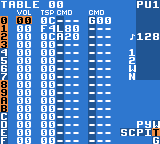
\includegraphics{table-slide}}
		\caption{Table Slide}
	\end{center}
\end{figure}

Transposes and slides are added together independently. In the above example, step 0 transposes one octave up. In step 1, the L command starts sliding one octave down while keeping the transpose from step 0 unchanged. In step 2, the L command is allowed to continue while the transpose stays one octave up. After some time, L will stop one octave down, canceling out the transpose and returning to the base note.

\section{M: Master Volume}

Changes the master output volume. The first digit modifies the left output, the second digit the right. The volume can either be set with an absolute value, or changed by a relative value.

Values 0-7 are used to specify absolute volumes. Values 8-\$F give the volume a relative change; 8 is no change, 9-\$B increase, \$D-\$F decrease.

\begin{description}
\item Examples:
\item[M77] maximize volume
\item[M08] minimize left volume, leave right volume unchanged
\item[M99] increase volume with 1 step
\item[MFE] decrease left volume with 1 step, right volume with 2 steps
\end{description}

\section{O: Set Output}

Pan channel to left, right, none or both outputs.

\section{P: Pitch Bend}

\subsection{For Pulse, Wave and Kit Instruments:}

Does a pitch change with the given speed. The behavior depends on the instrument's \textsc{pitch} setting:

\begin{description}
    \item[\textsc{drum}] Logarithmic pitch bend that updates at 360 Hz.
    \item[\textsc{fast}] Linear pitch bend that updates at 360 Hz.
    \item[\textsc{tick}] Pitch bend that updates every tick.
    \item[\textsc{step}] Immediate pitch change without bend.
\end{description}

Example:

\begin{description}
\item[P02] Pitch change up with speed 2.
\item[PFE] Pitch change down with speed 2. (\$FE=-2)
\end{description}

\subsection{For Noise Instruments:}

Applies S command with the given value every tick.

\section{R: Retrig/Resync}

Retrig plays the latest played note again. The first digit modulates the volume (0=no change, 1-7=increase, 9-\$F=decrease). The second digit sets retrig rate, 0 being the fastest and \$E the slowest, and \$F meaning only retrig once.

R8x means resync: With this option, the sound generator restarts at a very high rate. The pulse channels have a special quirk which makes resync slow down the sound, allowing it to go half an octave deeper.

\begin{description}
\item Example:
\item[R00] retrig the sound every tick
\item[R0F] retrig once
\item[R80] restart the sound generator at 360 Hz
\item[RF3] retrig the sound every fourth tick, decreasing amplitude (echo effect)
\end{description}

\section{S: Sweep/Shape}

This command has different effects for different instrument types.

\subsection{Pulse Instruments}

Frequency sweep, useful for bass drums and percussion. The first digit changes pitch, the second changes pitch change speed. Only works on the first pulse channel.

\subsection{Kit Instruments}

S changes the loop points. The first digit modulates the offset value; the second digit modulates the loop length. (1-7=increase, 9-\$F=decrease.) Used creatively, this command can be very useful for creating a wide range of percussive and timbral effects.

\subsection{Noise Instruments}

Alters noise shape (see section~\ref{noise-instrument-parameters}).
The command is relative, meaning that the digits are independently added to the active noise shape.

\section{T: Tempo}

Changes the tick rate to match the given beats per minute (BPM) value. The BPM is accurate only if the active groove has 6 ticks per note step. If the groove has some other number of ticks per note step, the BPM value should be adjusted according to the formula
\begin{math}
lsdj\_bpm = (desired\_bpm \times ticks\_per\_step)/{6}
\end{math}.
\textsc{t28}-\textsc{tff} selects 40-255 BPM, \textsc{t00}-\textsc{t27} selects 256-295 BPM.

\begin{description}
\item Example:
\item[T80] set tempo to 128 BPM
\item[TFF] set tempo to 255 BPM
\item[T27] set tempo to 295 BPM
\end{description}

\section{V: Vibrato}

Adds vibrato. Not available for noise instruments. The vibrato speed and shape depends on the instrument's \textsc{pitch} setting.
The first digit sets speed, second sets depth.

\begin{figure}[hbtp]
    \begin{tabular}{r|r|r|r|r|r|r|r|r}
        Depth & 0 & 1 & 2 & 3 & 4 & 5 & 6 & 7 \\
        \hline
        Semitones & 0.125 & 0.25 & 0.375 & 0.5 & 0.75 & 1 & 1.5 & 2 \\
    \end{tabular}

    \begin{tabular}{r|r|r|r|r|r|r|r|r}
        Depth & 8 & 9 & A & B & C & D & E & F \\
        \hline
        Semitones & 2.5 & 3 & 3.5 & 4 & 5 & 6 & 7 & 8 \\
    \end{tabular}
\end{figure}

\begin{description}
\item Example:
\item[V42] speed=4, depth=0.375 semitones
\item[V00] reset vibrato
\end{description}

\section{W: Wave}

\subsection{For Pulse Instruments:}
Changes waveform. Due to a hardware oddity, the instrument \textsc{length} timer is reset, possibly extending the duration of the sound.

\subsection{For Wave Instruments:}
The first digit sets synth sound speed, the second sets synth sound length. 0 = no change. The synth restarts if length is changed.

\section{Z: RandomiZe}

The Z command repeats the last command that is not Z or H, adding a random number to the original command value. The Z value controls the maximum value of each digit to be added.

\begin{description}
\item Example:
\item[Z02] adds one of 0, 1, 2 to the original value.
\item[Z20] adds one of 0, 10, 20 to the original value.
\item[Z22] adds one of 0, 1, 2, 10, 11, 12, 20, 21, 22 to the original value.
\end{description}
